% ........................................................................... %

We give here some background knowledge on timed automata that will be useful for the remainder of this work. More precisely, we first present the model ands its semantics. We then focus on the closure properties of timed automata operators (e.g., intersection, complementation, ...). We recall and explain the important results on the decidability of the reachability and language inclusion problems. We give an overview of the main timed automata classes and extensions as well as their properties regarding the aforementioned closure and decidability problems. Finally, we explain how timed automata are used for performing model checking tasks, and we present the related tools.\\

% ........................................................................... %

\section{Model and semantics}

% ........................................................................... %

\subsection{Timed automata}

% ........................................................................... %

Timed automata were introduced in \cite{RADLD94} as an extension of classical automata \cite{Hopcroft79} to model real-time systems. Some preliminary works appeared in \cite{RACC94}. They add real-valued clocks to automata. The clocks of a timed automaton evolve synchronously and continuously as time elapses. Clocks can be used to create constraints called \emph{guards} that specify when a switch can be fired. Also, a subset of clocks can be \emph{reset} to zero when a switch is fired. Time elapses in the locations, while the switches are instantaneous. It is also possible to bound the time spent in the locations by defining clocks constraints called \emph{invariants}, which can be used to force switches to be fired before the invariants conditions become violated. Indeed, it is a requirement that time can always elapse in the locations. Timed automata recognize \emph{timed words} which are sequences in which a non-negative real value is attached to each symbol. For example $w = (a, 0) \cdot (b, 1)$ is a timed word where $b$ has been recognized 1 unit of time after $a$. More precisely, a timed word over an alphabet $\Sigma$ is a sequence $(a_0,t_0) \cdot (a_1, t_1) \cdots (a_n, t_n)$ such that $a_i \in \Sigma$,  $t_i \in \Rpos$ and  $t_0 < t_1 < \cdots < t_n$.\\

Given a set of clocks $X$ with their values being in $\Rpos$, a clocks valuation $v$ for $X$ is a function $X \longrightarrow \Rpos$ that associates to each clock $x \in X$ its value $v(x)$. The set of clocks valuations for $X$ is written $\Rpos^X$. The set of clocks constraints over $X$ is $\mathcal{C}(X)$, built using boolean combinations of atomic constraints of the form $x \;\#\; c$ with $x \in X$, $\;\#\; \in \{=, \neq, <, \leq, >, \geq \}$ and $c \in \Qpos$. $\mathcal{C}_{\prec}(X)$ is the restrictions of $\mathcal{C}(X)$ where the clocks constraints are of the form $x < c$ or $x \leq c$. A clocks valuation $v$ satisfies an atomic constraint $x \;\#\; c$ if and only if $v(x) \;\#\; c$. This allows to check whether a complete constraint $g$ can be satisfied by a clocks valuation $v$, denoted as $v \models g$. Given $d \in \Rpos$, $v' = v + d$ is the clocks valuation such that $v'(x) = v(x) + d$ for each $x \in X$. Also, given a subset of clocks $r \in X$, $v' = [r \leftarrow 0]v$ is the clocks valuation such that $v'(x) = 0$ if $x \in r$ and $v'(x) = v(x)$ if $x \in X \setminus r$.

\begin{definition}[Timed automata] \cite{RADLD94,RA98}
  
A timed automaton $A$ is a tuple $A = (L, L^0, L^f, X, I, E, \Sigma)$ where:
\begin{itemize}

    \item $L$ is a finite set of \emph{locations} (or states),

    \item $L^0 \subseteq L$ is the set of \emph{initial locations},

    \item $L^f \subseteq L$ is the set of \emph{final locations} (or accepting states),

    \item $X$ is a finite set of clocks,

    \item $I : L \rightarrow \mathcal{C}_{\prec}(X)$ associates an \emph{invariant} to each location

    \item $E \subseteq L \times \mathcal{C}(X) \times \Sigma \times 2^X \times L$ is a finite set of switches (or switches) $e = (l, g, a, r, l') \in E$ from $l$ to $l'$, where $g$ is the guard, $r$ is the set of clocks to be reset and $a$ is the label,

    \item $\Sigma$ is the \emph{alphabet}.

\end{itemize}
\end{definition}

\begin{figure}[htbp]
    \centering
    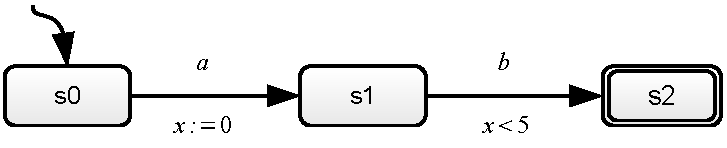
\includegraphics[width=0.9\textwidth]{content/timed-automata/sample-ta}
    \caption{A sample timed automaton $A$.}
    \label{fig:sample-ta}
\end{figure}

The timed automaton $A$ depicted on Figure~\ref{fig:sample-ta} uses one clock $x$ which is reset to $0$ when the automaton switches from the location $s_0$ to $s_1$ on the symbol $a$. The clock $x$ is  also used in the guard of the switch which recognizes $b$ to specify that the automaton $A$  recognizes only  timed words  $(a, t) \cdot (b, t') $ with $t' - t < 5$ (i.e., the set of words $a \cdot b$ such that $b$ is recognized at most 5 units of time after $a$).

% ........................................................................... %

\subsection{Semantics}

% ........................................................................... %

The semantic of a timed automaton $A$ is defined using an (infinite) timed \emph{labeled transitions system} (LTS). Each state of the LTS is a pair $(l, v) \in L \times \Rpos^X$, called a \emph{configuration}, where $l$ is the current location in $A$ and $v$ is a clocks valuation. There are two types of transitions: \emph{action transitions} (labeled with a symbol of $\Sigma$) and \emph{time transitions} (labeled with a real-valued duration). More precisely, the semantic of $A = (L, L^0, L^f, X, I, E, \Sigma)$ is given by the LTS $\mathcal{S}_A = (S, s_0, \rightarrow, \Sigma)$ where:

\begin{itemize}

    \item $S = L \times \Rpos^X$,

    \item $s_0 = (l_0, v_0)$ with $l_0 \in L^0$ and $v_0(x) = 0$ $\forall x \in X$,

    \item $\rightarrow$ is the transition relation:
    \begin{itemize}

        \item action transitions: $(l, v) \stackrel{a}{\longrightarrow} (l', v')$ if and only if there exists
        $e = (l, g, a, r, l') \in E$ such that $v \models g$, $v' = [r \leftarrow 0]v$ and $v' \models I(l')$

        \item time transitions: if $d \in \Rpos$ then $(l, v) \stackrel{d}{\longrightarrow} (l, v + d)$ if and only if $v + d \models I(l)$.

    \end{itemize}

\end{itemize}

The LTS $\mathcal{S}_A$ starts from an initial state made from an initial location and each clock set to $0$. Then, either instantaneous action transitions occur (possibly resetting some clocks), or time transitions allow the clocks to grow synchronously. The executions over $\mathcal{S}_A$ match the timed words that can be recognized by $A$ when they start from the initial state of $\mathcal{S}_A$ and they can reach a final state.\\

\begin{figure}[htbp]
    \centering
    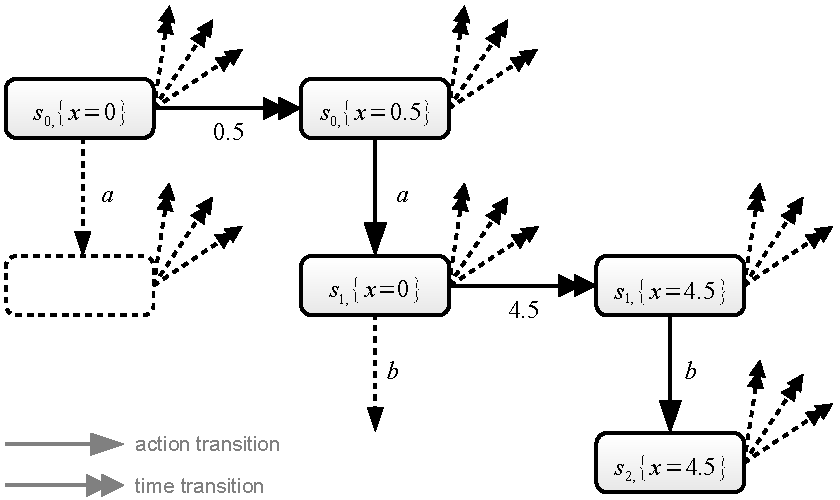
\includegraphics[width=\textwidth]{content/timed-automata/semantic-lts}
    \caption{The LTS $\mathcal{S}_A$ associated to the timed automaton $A$ of Figure~\ref{fig:sample-ta}.}
    \label{fig:semantic-lts}
\end{figure}

Let us consider again $A$ defined on Figure~\ref{fig:sample-ta} and its semantic LTS $\mathcal{S}_A$ which is depicted on Figure~\ref{fig:semantic-lts}. $(s_0, 0) \stackrel{1}{\longrightarrow} (s_0, 1) \stackrel{0.25}{\longrightarrow} (s_0, 1.25) \stackrel{a}{\longrightarrow} (s_1, 0) \stackrel{0.1}{\longrightarrow} (s_1, 0.1) \stackrel{b}{\longrightarrow} (s_2, 0.1)$ is a valid execution over $\mathcal{S}_A$ which recognizes the timed word $(a, 1.25) \cdot (b, 1.35)$ of the timed language $L(A)$.

% ........................................................................... %

\subsection{Deterministic timed automata}

% ........................................................................... %

The definition of timed automata supports indeterminism as a given timed word may support more than one run over an automaton. Let us consider the timed automaton depicted on Figure~\ref{fig:indeterministic-ta}: the timed word $(a, 0) \cdot (a, 0.52) \cdot (a, 5)$ supports two accepting runs. One ends in the state $s_1$ while the other ends in the state $s_2$.\\

\begin{figure}[htbp]
    \centering
    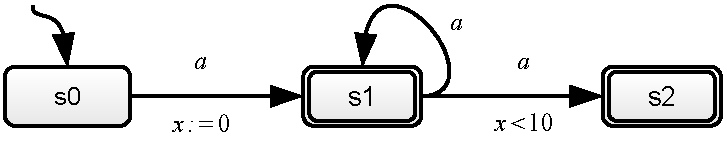
\includegraphics[width=0.9\textwidth]{content/timed-automata/indeterministic-ta}
    \caption{An indeterministic timed automaton.}
    \label{fig:indeterministic-ta}
\end{figure}

The class of \emph{deterministic timed automata} has been defined in \cite{RADLD94}. Each timed word that is recognized by a deterministic timed automaton has exactly one accepting run over it. Deterministic timed automata form a strict subclass of timed automata (they are less expressive). The problem of the determinization of indeterministic (untimed) automata is decidable \cite{Hopcroft79}. This is however not the case for timed automata \cite{ST03}.

\begin{definition}[Deterministic timed automata] \cite{RADLD94,RA98}

A timed automaton $A = (L, L^0, L^f, X, I, E, \Sigma)$ is \emph{deterministic} if and only if:
\begin{enumerate}

	\item $|L^0|=1$ (it has only one initial location), and

	\item for all switches $e_1 = (l_1, g_1, a_1, r_1, l_1')$ and $e_2 = (l_2, g_2, a_2, r_2, l_2')$ in $E$ such that $l_1 = l_2$ and $a_1 = a_2$ then there is no clocks valuation $v$ such that both $v \models g_1$ and $v \models g_2$.

\end{enumerate}
\end{definition}

% ........................................................................... %

\section{Closure properties}

% ........................................................................... %

Closure of timed automata under the following operators has been studied.
\begin{description}

	\item[Union and intersection.]\

	Computing the union or the intersection of timed automata is achieved by using an extended automata product construction \cite{Hopcroft79,RADLD94}.

	\item[Complementation.]\

	The complement of a timed automaton $A$ recognizes the complement of the timed language $\mathcal{L}(A)$. As we will see, this construction is not decidable for indeterministic timed automata.

	\item[Projection.]\

	The projection allows to map a timed language to another one that supports a different alphabet. This can be achieved by using $\varepsilon$ as a label on every switch where the original label does not belong to the new alphabet.

\end{description}

\begin{theorem} \cite{RADLD94,RA98}
  
The set of timed regular languages is closed under union, intersection and projection, but not under complementation.

\end{theorem}

The case of deterministic timed automata is slightly different. Indeed, every timed word accepts exactly one run over the timed automaton that recognizes its timed language. This property allows to compute the complement of timed automaton. The case of projection is also different, as the removal of $\varepsilon$ transitions can lead to indeterminism, hence deterministic timed automata are not closed under projection. The case of union and intersection remains unchanged.

\begin{theorem} \cite{RADLD94,RA98}
  
Deterministic timed automata are closed under union, intersection and complementation, but not under projection.

\end{theorem}

% ........................................................................... %

\section{Reachability analysis}

% ........................................................................... %

Reachability analysis is an essential technique for performing verification on timed automata. Given a timed automaton $A$, the following two dual problems have been studied.
\begin{enumerate}

	\item The \emph{reachability problem} consists in checking whether a final location $l_f$ of $A$ can be reached by an execution of a timed word of $\mathcal{L}(A)$ from an initial location $l_0$ to $l_f$. Such an execution must be identified in the labeled transition system $\mathcal{S}_A$ which is infinite in the number of states.

	\item The \emph{emptiness problem} consists in checking whether the timed language $\mathcal{L}(A)$ is empty or not. The language is said to be empty when there is not timed word that supports an accepting run over $A$. This problem reduces to the reachability problem as $\mathcal{L}(A)$ is not empty as long as at least one of its final location can be reached from an initial location through a timed word execution over it.

\end{enumerate}

Given that the number of states of $\mathcal{S}_A$ is infinite, it is not possible for an algorithm to manipulate it directly. The solution that we briefly recall below is to:
\begin{enumerate}

	\item define a partitioning of $\mathcal{S}_A$

	\item build a time-abstract automaton from the partitioning

	\item reduce the reachability problem in $\mathcal{S}_A$ to a reachability problem in the obtained time-abstract automaton.
\end{enumerate}

% ........................................................................... %

\subsection{Partitioning of $\mathcal{S}_A$}

% ........................................................................... %

The idea of the partitioning of $\mathcal{S}_A$ is to group the configurations of $\mathcal{S}_A$ that are equivalent from a behavioral point of view. The number of theses groups, called \emph{clock regions} is finite, yet exponential in the encoding of the clock constraints and invariants of $A$ (the larger the constants are, the larger the number of clock regions is). The construction of clock regions is made by grouping the states of $\mathcal{S}_A$ (the configurations) using the following equivalence relation.\\

The guards and invariants of $A$ are supposed to use only integer constants. If not, then they can be simply multiplied by the least-common-multiple of all the constant denominators. Indeed, the definition of timed automata requires the constants to be rational. Multiplying the constants of a guards and invariants of a timed automaton by the same factor does not change the recognized timed language (modulo the multiplication of the event dates!). Given a real value $r \in \R$, we denote as $\lfloor r \rfloor$ its integral part and $\{r\}$ as its fractional part (e.g., $\lfloor 1.25 \rfloor = 1$ and $\{1.25\} = 0.25$). For each clock $x \in X$ of $A$, we denote as $c_x$ the largest integer to which $x$ is compared.

\begin{definition}[Clock region] \cite{RADLD94,RA98}

Two configurations $(l, v)$ and $(l', v')$ are equivalent (denoted as $(l,v) \cong (l',v')$) if $l = l'$, and
\begin{enumerate}

  \item $\forall x \in X$ either $\lfloor v(x) \rfloor = \lfloor v'(x) \rfloor$ or both $v(x) > c_x$ and $v'(x) > c_x$

  \item $\forall x,y \in X$ such as $v(x) \leq c_x$ and $v(y) \leq c_y$, then $\{v(x)\} \leq \{v(y)\}$ if and only if $\{v'(x)\} \leq \{v'(y)\}$

  \item $\forall x \in X$ such as $v(x) \leq c_x$, $\{v(x)\} = 0$ if and only if $\{v(x)\} = 0$.

\end{enumerate}
\end{definition}

The condition on the location names to be equal is no surprise. The first two conditions on the clocks valuation require that two valuations can only be equivalent if they satisfy the same constraints. The third one ensures that the clocks will change their integral parts \emph{in the same order}.
%
The regions can be constructed by generating all the clock regions combinations using the following procedure:
\begin{enumerate}

	\item for each clock $x \in X$, we pick a clock constraint in the set
	$$   \left\{ x = c \;|\; c = 0, 1, \cdots, c_x \right\}
	\cup \left\{ c - 1 < x < c \;|\; c = 1, \cdots, c_x \right\}
	\cup \left\{ x > c_x \right\}
	$$

	\item for every pair of clocks $x, y \in X$ and $c, d \in \N$ such that $c - 1 < x < c$ and $d - 1 < y < d$ appear in the clock constraints chosen above, we add a constraint to state whether $\{x\} < \{y\}$, $\{x\} = \{y\}$ or $\{x\} > \{y\}$.

\end{enumerate}

\begin{lemma} \cite{RADLD94}
  
The number of clocks regions is bounded by
$$
|X|! \cdot 2^{|X|} \cdot \prod\limits_{x \in X}(2c_x + 2)
$$
where $X$ is the set of clocks and given $x \in X$, $c_x$ is the largest constant to which it is compared to.
\end{lemma}

\begin{figure}[htbp]
		\centering
    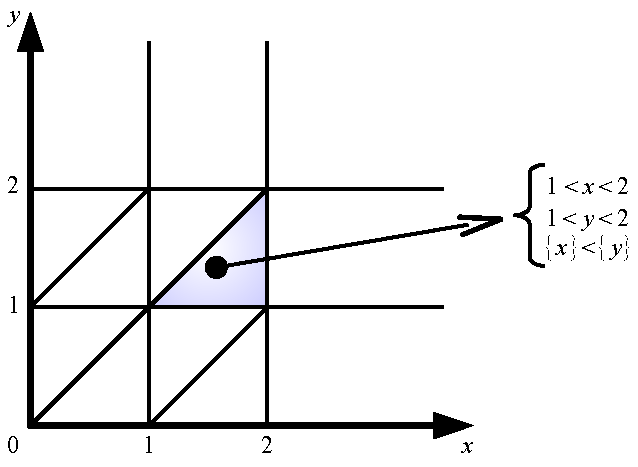
\includegraphics[width=0.8\textwidth]{content/timed-automata/region-clocks}
    \begin{flushright}
    	\textit{(source: \cite{BL-VAT06})}
    \end{flushright}
    \caption{Region clocks.}
    \label{fig:region-clocks}
\end{figure}

Let us consider the case of two clocks $x$ and $y$ such as the biggest constant to which both are compared is 2. Figure~\ref{fig:region-clocks} shows a representation of the clocks regions.

% ........................................................................... %

\subsection{Region automata}

% ........................................................................... %

Using the equivalence relation $\cong$, it is possible to build the \emph{region automaton} $R_A$ of a timed automaton $A$. This automaton is time-abstract: the states represent the clock regions and the transitions are made on the words of the alphabet of $A$.

\begin{definition}[Region automaton] \cite{RADLD94,RA98}

Let $A$ be a timed automaton. Its region automaton $R_A$ is built as follows.
\begin{itemize}

  \item The states of $R_A$ are the pairs $(l, r)$ where $l$ is a location of $A$ and $r$ a clocks region obtained using $\cong$.

  \item A transition $(l, r) \xrightarrow{a} (l', r')$ is added when there exists $l \xrightarrow{g, a, Y := 0} l' \in A$, a clocks valuation $v \in r$ and $t \geq 0$ such that
  \begin{enumerate}

    \item $v + t \models I(l)$, and

    \item $v + t \models g$, and

    \item $[Y \leftarrow 0](v + t) \models I(l')$, and

    \item $[Y \leftarrow 0](v + t) \models I(l') \in r'$.

  \end{enumerate}

  \item The initial (respectively final) states of $R_A$ correspond to the states $(l, r)$ such that $l$ is an initial (respectively final) location of $A$.

\end{itemize}
\end{definition}

\begin{figure}[htbp]
    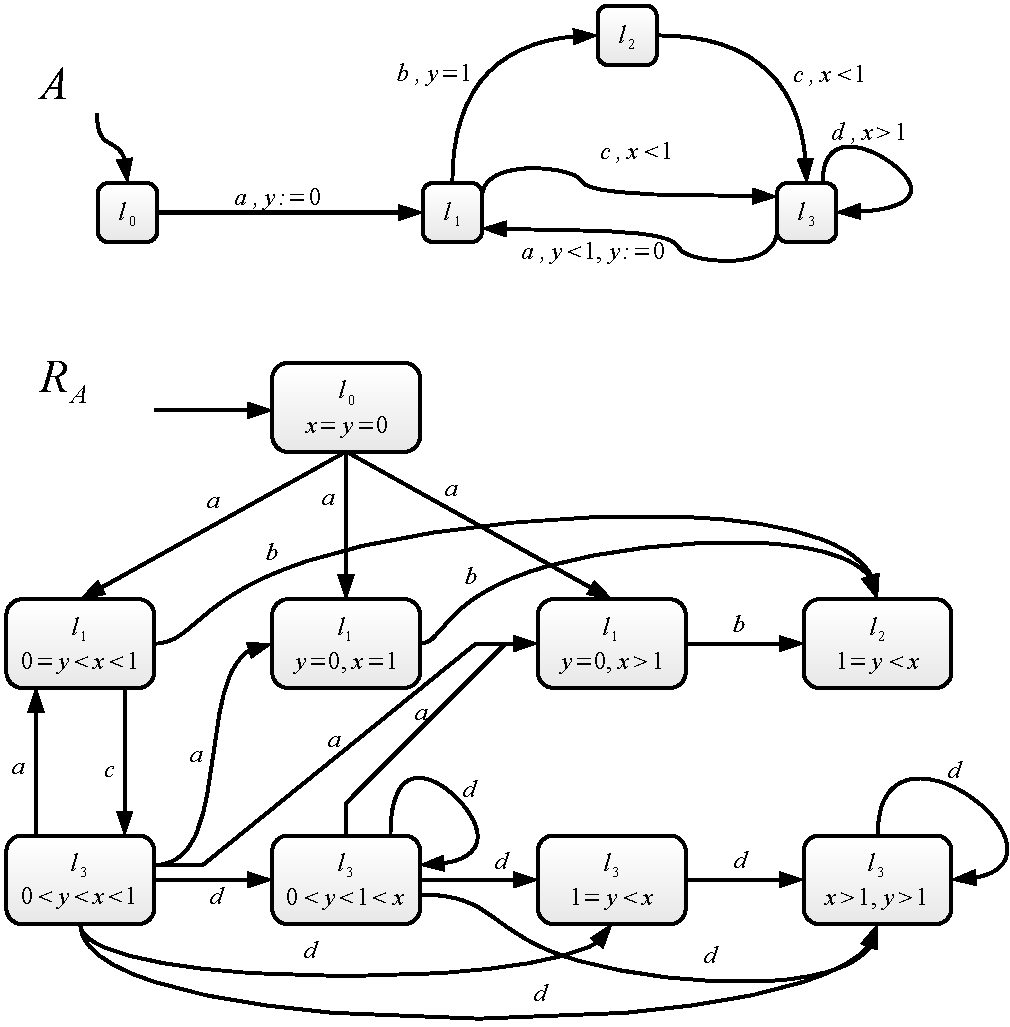
\includegraphics[width=\textwidth]{content/timed-automata/region-automaton}
    \begin{flushright}
    	\textit{(source: \cite{RADLD94})}
    \end{flushright}
    \caption{A timed automaton $A$ and its associated region automaton $R_A$.}
    \label{fig:region-automaton}
\end{figure}

$R_A$ recognizes the words $w = (a_0) \cdot (a_1) \cdots (a_n)$ such that there exists a timed word $w_t = (a_0, t_0) \cdot (a_1, t_1) \cdots (a_n, t_n)$ that is recognized by $A$. As a consequence, the reachability problem in $A$ reduces to a reachability problem in $R_A$ \cite{RADLD94}. An example of a timed automaton and its region automaton is given in Figure~\ref{fig:region-automaton}.

\begin{theorem} \cite{RADLD94}
  
The reachability and emptiness checking problems for timed automata are \textsc{PSPACE-Complete}.

\end{theorem}

The exact time complexity is $\mathcal{O}\left(m \cdot k! \cdot 4^k \cdot (c \cdot c' + 1)^k\right)$ where $m$ is the number of switches in $A$, $k$ is the number of clocks in $A$, $c$ is the largest numerator in the constants of the guards and invariants in $A$ and $c'$ is the least-common-multiple of the denominators of all the constants of the guards and invariants in $A$ \cite{RADLD94}.

% ........................................................................... %

\section{Timed language inclusion, equivalence and universality}

% ........................................................................... %

We briefly introduce these three decision problems.
%
Given two timed automata $A$ and $A'$, the \emph{timed language inclusion problem} refers to checking if $\mathcal{L}(A) \subset \mathcal{L}(A')$. Similarly, the \emph{timed language equivalence problem} refers to checking if $\mathcal{L}(A) = \mathcal{L}(A')$. Finally, the \emph{universality problem} refers to checking whether a timed automaton $A$ defined over an alphabet $\Sigma$ is able to recognize all of the possible timed words over $\Sigma$.\\

These problems require the ability to complement timed automata. As an example, checking whether $\mathcal{L}(A) \subset \mathcal{L}(A')$ reduces to checking for the timed language emptiness of the automaton $A' \cap \overline{A}$. Unfortunately, timed automata are not closed under complementation, making these problems undecidable.

\begin{theorem} \cite{RADLD94}
  
The inclusion, equivalence and universality problems for timed automata are undecidable.

\end{theorem}

The case of deterministic timed automata is more interesting as they are closed under complementation, making these problems decidable, yet \textsc{Pspace}-complete.

\begin{theorem} \cite{RADLD94}

The inclusion, equivalence and universality problems for deterministic timed automata are \textsc{Pspace}-complete.

\end{theorem}

% ........................................................................... %

\section{Classes and extensions}

% ........................................................................... %

\begin{table}[htbp]
\centering
\footnotesize
\begin{tabular}{|p{5cm}|p{4.5cm}|p{2.5cm}|}

	\hline
	
	\textit{Class or extension} &
	\textit{Emptiness checking} &
	\textit{Language inclusion} \\
	
	\hline \hline
	
	  Timed automata &
    \textsc{PSPACE-Complete} &
    Undecidable \\

    \hline

    Deterministic timed automata &
    \textsc{PSPACE-Complete} &
    Decidable \\

    \hline

    Event-clock automata &
    \textsc{PSPACE-Complete} &
    Decidable \\

    \hline

    Robust timed automata &
    \textsc{PSPACE-Complete} &
    Undecidable \\

    \hline \hline

    $\varepsilon$-transitions without clocks resets &
    \textsc{PSPACE-Complete} &
    Undecidable \\

    \hline

    $\varepsilon$-transitions with clocks resets &
    \textsc{PSPACE-Complete} &
    Undecidable \\

    \hline

    Diagonal constraints ($x - y \;\#\; c$)&
    \textsc{PSPACE-Complete} &
    Undecidable \\

    \hline

    Additive constraints ($x + y \;\#\; c$) &
    Decidable for 1 or 2 clocks, open problem for 3 clocks and undecidable starting from 4 clocks \cite{BerDuf-IPL2000} &
    Undecidable \\

    \hline
    
    Constraints of the form $x = 2y$ &
    Undecidable \cite{RADLD94} &
    Undecidable \\
    
    \hline
    
    Constraints with irrational constants &
    Undecidable \cite{Miller00} &
    Undecidable \\

    \hline

    Non-standard ($x := 0$) clocks resets &
    Decidable for $x := c$, undecidable for $x := x -1$ and decidable for $x := x + 1$ if diagonal constraints are not allowed \cite{BDFP04} &
    Undecidable \\
    
    \hline

\end{tabular}
\caption{Emptiness and timed language inclusion checking results for some classes and extensions of timed automata.}
\label{tab:ta-classes-decidability}
\end{table}

\begin{table}[htbp]
\centering
\footnotesize
\begin{tabular}{|p{5cm}|p{7.5cm}|}

    \hline

    \textit{Class or extension} &
    \textit{Expressiveness} \\

    \hline \hline

    Timed automata &
		-- \\
		
    \hline

    Deterministic timed automata &
    Strictly less expressive than timed automata \\

    \hline

    Event-clock automata &
    Indeterministic event-clock automata can always be rendered deterministic while this is not the case for (general) timed automata \cite{RALF94} \\

    \hline

    Robust timed automata &
    Robust timed languages are \emph{open} and their expressiveness is not comparable with the one of timed languages \cite{RAPM04} \\

    \hline \hline

    $\varepsilon$-transitions without clocks resets &
    The silent transitions can be removed \cite{VDPG97} \\

    \hline

    $\varepsilon$-transitions with clocks resets &
    Strictly more expressive than general timed automata: the silent transitions that reset clocks cannot be removed in general \cite{VDPG97,BBVD+99,LSV:07:12} \\

    \hline

    Diagonal constraints ($x - y \;\#\; c$)&
    More concise than timed automata, but not more expressive \cite{BBVD+99} \\

    \hline

    Additive constraints ($x + y \;\#\; c$) &
    More expressive than timed automata \\

    \hline
    
    Constraints of the form $x = 2y$ &
    -- \\
    
    \hline
    
    Constraints with irrational constants &
    -- \\

    \hline

    Non-standard ($x := 0$) clocks resets &
    -- \\

    \hline

\end{tabular}
\begin{flushleft}
	\emph{Note: a ``--'' means that there is nothing special compared to general timed automata.}
\end{flushleft}
\caption{Expressiveness of some classes and extensions of timed automata.}
\label{tab:ta-classes-expressiveness}
\end{table}

Several classes and extensions of timed automata have been studied. Indeed, the fact that the decision problems seen above are undecidable in the general case motivated such research directions. We summarize here the principal classes and extensions of timed automata that turned out to be useful in the context of this work.
%
Table~\ref{tab:ta-classes-decidability} summarizes the results regarding the timed language inclusion and emptiness checking problems, while Table~\ref{tab:ta-classes-expressiveness} details the results on expressiveness.
%
Further pointers can be found in \cite{RAPM04,RA98,ST03,JOJW04,BL-VAT06}.\\

Some classes or extensions have different expressiveness levels compared to (general) timed automata. The expressiveness of the class of \emph{Robust timed automata} cannot be compared to the one of timed automata \cite{RAPM04}. Briefly, a robust timed automaton allows to recognize a timed word with some fuzziness in the event dates. Indeed, no real world system can be expected to be as precise as timed automata expect them to be. The classical decidability problems (reachability / emptiness, inclusion) remain unchanged.
%
Allowing silent ($\varepsilon$) transitions strictly adds to the expressiveness \cite{VDPG97,BBVD+99,LSV:07:12}. In the case of untimed automata, they do not add to the expressiveness and they can be removed. This is however not the case with timed automata. Techniques exist to remove the $\varepsilon$-transitions when they not reset clocks \cite{VDPG97}. However, this is not possible when they do reset clocks, i.e., there exist switches of the form $l \xrightarrow{\varepsilon, g, \{ x \}} l'$.\\

It is interesting to note that the timed language inclusion problem is only decidable in the case of deterministic timed automata and \emph{event-clock automata}, a class where each word of the alphabet is associated to a clock which is reset whenever it is recognized \cite{RALF94}. In fact, an indeterministic timed automaton can always be transformed into a deterministic timed automaton.\\

In many cases, the emptiness / reachability problems are decidable (yet \textsc{Pspace}-complete) despite the language inclusion problem being undecidable because of a non-closure under complementation. However, some forms of modified clocks constraints and clocks resets can render it undecidable \cite{BerDuf-IPL2000,RADLD94,Miller00,BDFP04,BBVD+99,LSV:07:12,VDPG97}.

% ........................................................................... %

\section{Model checking using timed automata}

% ........................................................................... %

\subsection{Principle}

% ........................................................................... %

\begin{figure}[htbp]
    \centering
    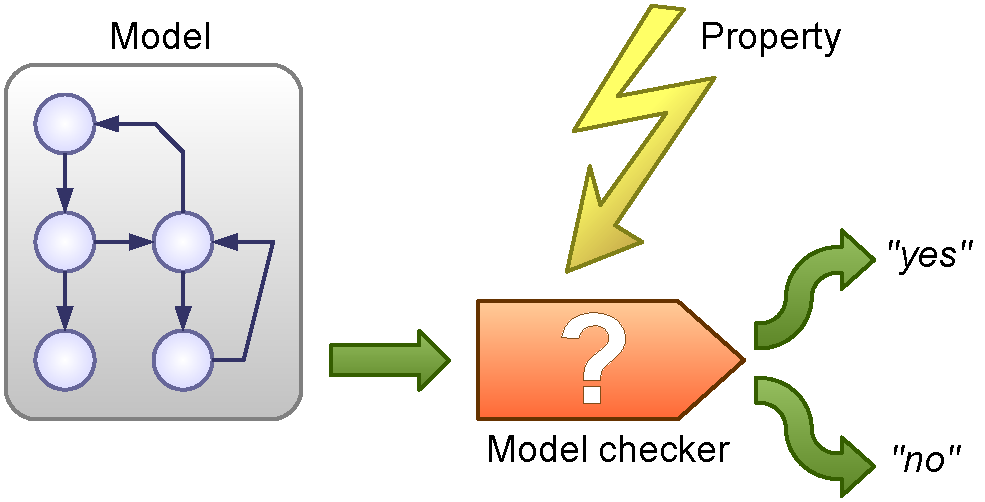
\includegraphics[width=0.9\textwidth]{content/timed-automata/model-checking}
    \caption{Principle of model checking.}
    \label{fig:model-checking}
\end{figure}

We briefly introduce the general principle of \emph{model checking} that we illustrated on Figure~\ref{fig:model-checking}. It refers to the process of testing \emph{properties} of a system for which a \emph{model} is given. The \emph{model checker} is a ``black box'' component that takes both of them as inputs then outputs whether the property is satisfied or not. Some model checkers can also output a \emph{trace}, mostly to give details of why the property cannot be satisfied (they are sometimes referred as \emph{error traces}).\\

The types of properties to be checked are usually classified in the following categories, although a model checker does not especially distinguish them.
\begin{description}
  
  \item[Reachability properties] checks wether a property can possibly be satisfied by the system. An example would be \emph{``the light can be switched off''}.
  
  \item[Safety properties] state that something which is considered as ``bad'' will never happen in the system. Continuing with the previous example, such a property could be \emph{``the light cannot stay on for more than 20 minutes''}.
  
  \item[Liveness properties] state that something which is considered as ``good'' will eventually happen. In the case of a system that can be executed infinitely, it also specifies that the property will always be able to happen. An example here would be \emph{``when the light is off, pressing the button turns it on''}.
  
\end{description}

In the case of timed automata, these verifications can be done in 2 ways:
\begin{enumerate}
  
  \item by reduction of timed language inclusion to a reachability / emptiness analysis, or
  
  \item by using a quantitative-time extension of linear or branching temporal logics.
  
\end{enumerate}

We now give an overview of these types of verifications.\\

% ........................................................................... %

\subsection{Verification through test automata}

% ........................................................................... %

In this case, the property to verify is expressed as a timed automaton, referred to as a \emph{test timed automaton}. The verification is performed by a reduction to a reachability / emptiness analysis that can be done on region automata using the techniques that we saw above. \\

\begin{figure}[htbp]
    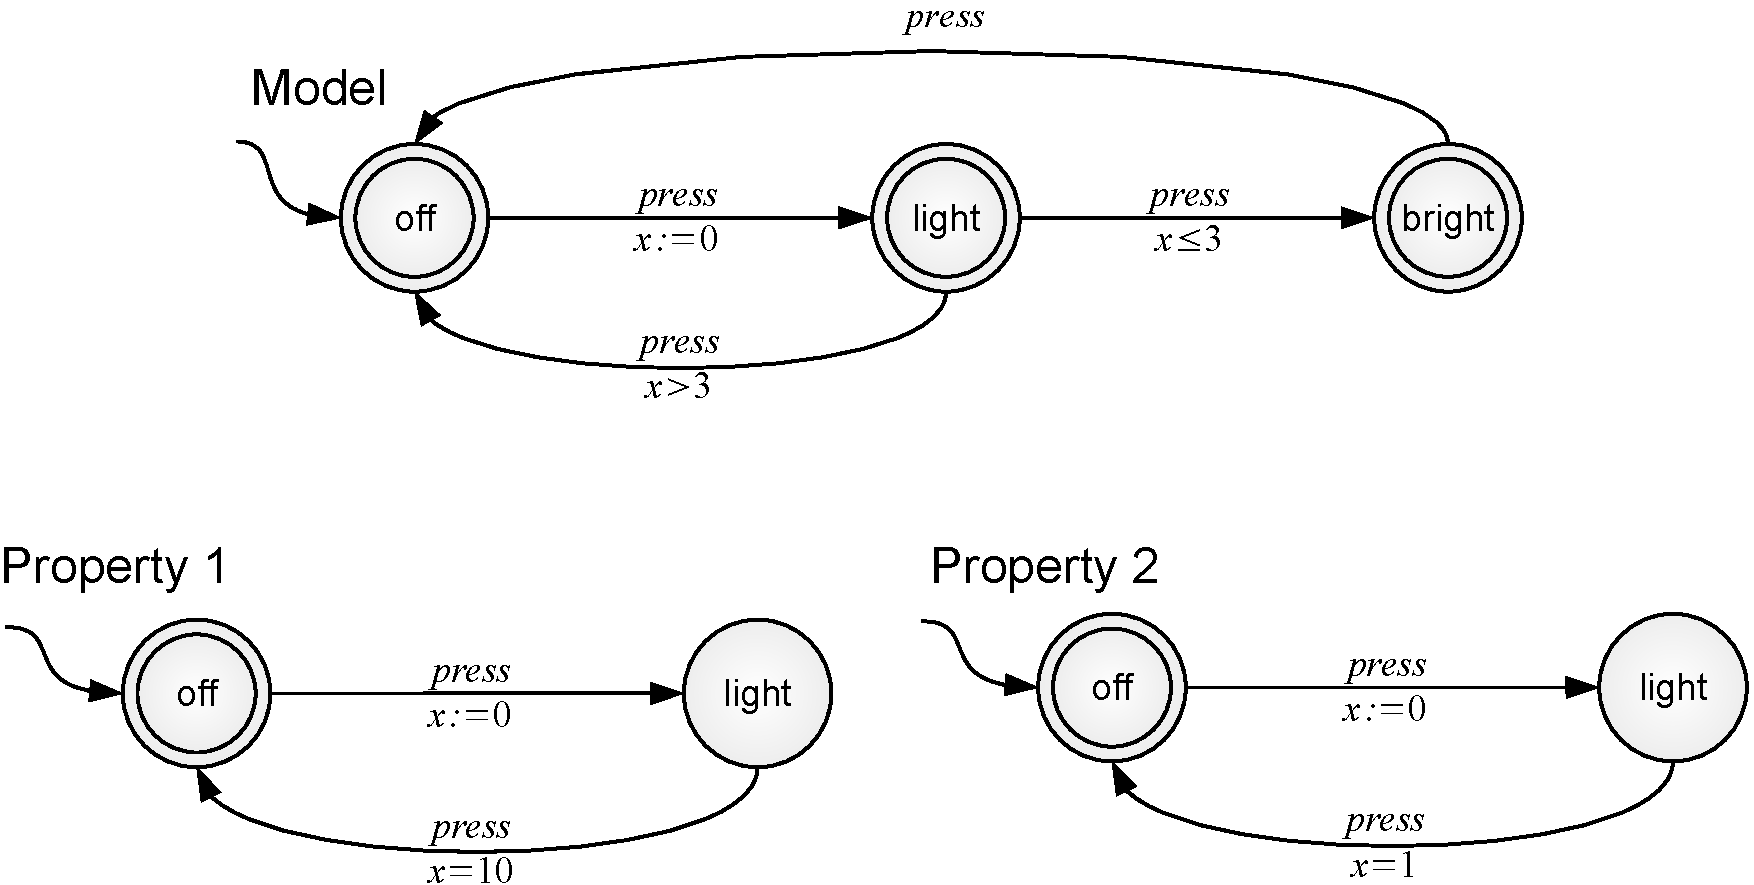
\includegraphics[width=\textwidth]{content/timed-automata/light-verification-inclusion}

    \begin{flushright}
    (\textit{model from} \url{http://www.cis.upenn.edu/~alur/Talks/sfm-rt-04.ppt})
    \end{flushright}

    \caption{A model checking example that reduces to state reachability analysis.}
    \label{fig:light-verification-inclusion}
\end{figure}

We give an example on Figure~\ref{fig:light-verification-inclusion}. The system that is modeled is a light controller. The light is initially turned off, and pressing it will turn it on. However, if the button is pressed twice quickly (at most 3 units of time), then the light will be brighter. Finally, pressing the button another time will turn the light off.\\

We express two properties on this system using timed automata. The first one (property one) is used to test whether pressing the button once, then 10 units of time later will turn it off again. This is property that we expect to be satisfied by the modeled system. In turn, we do not expect the second property to be true: when pressed quickly twice, the light should not be turned off.\\

Both properties can be tested against the timed language inclusion of the properties timed languages into the model timed language. Indeed, the timed automata are deterministic, hence they can be complemented and the problem reduces to a emptiness / reachability problem. In this case, the timed language that corresponds to the first property is indeed included in the one of the model timed language, hence the property is verified. Similarly, the second property is not verified as there is no timed language inclusion.\\

Model-checking through the mean of test automata is not always the best option. Indeed, modeling a property as a timed automaton may not always be easy: it must be encoded as the set of timed words to be allowed or forbidden. This can prove to be a time-consuming task during the model-checking assisted development of a hardware or software component, especially if the modeled system is frequently updated as each change may also need the test automata to be adapted. This may also hinder factorizing properties to be tested on several systems, with the worst case requiring each property to be adapted to each system.\\

Finally, the biggest limitation of test automata is that the verification may not always be possible as it reduces to a timed language inclusion checking problem. While checking for timed language emptiness is decidable for most classes and extensions (yet \textsc{PSPACE-Complete}), several classes of timed automata are not closed under complementation, including the general class of (indeterministic) timed automata \cite{RADLD94}. As a consequence, this technique is best used on classes with ``good'' properties such as deterministic timed automata \cite{RADLD94} or event-clock automata \cite{RALF94}.\\

A more popular technique is to express properties using temporal logics. As we will see, it is decidable in more cases, including general timed automata.\\

% ........................................................................... %

\subsection{Verification using temporal logics}

% ........................................................................... %


\emph{Temporal logics} have been traditionally used for formal verification purposes. A temporal logic formula typically expresses some form of \emph{qualitative time} property such as \emph{``when the light is off, pressing the button will turn it on''}. To put it another way, temporal logics allow to specify the order of events. However, it is not possible to express \emph{quantitative time} properties such as \emph{``when the light is off and the button is pressed twice in less than 2 seconds, the light will be bright''}.\\

The purpose of a temporal logic formula is to check wether there exists a path to a state that satisfies the formula in the considered system. For example, in the case of classical automata the state space is exactly the set of states of the considered automaton. We distinguish two types of temporal logics:
\begin{enumerate}
  
  \item \emph{linear-time temporal logics} allow reasoning over a single time line
  
  \item \emph{branching-time temporal logics} allow reasoning over several time lines.
  
\end{enumerate}
CTL, which stands for \emph{computational tree logic}, is the traditional branching-time logic \cite{ClarkeES86} while LTL (emph{linear temporal logic}) is the traditional linear-time logic \cite{Pnueli77}.\\

Both CTL and LTL have been extended to support quantitative time. TCTL (\emph{timed computational tree logic}) \cite{HNSY94} extends the branching-time logic CTL. Similarly, MTL (\emph{metric temporal logic}) \cite{Koymans90} and TPTL (\emph{timed propositional temporal logic}) \cite{AlurH89,AlurH94} extend the linear-time temporal logic LTL to support quantitative time. As we will see hereafter, some fragments of MTL have been defined to seek better decidability results: as MITL (\emph{metric interval logic}) \cite{AlurFH96}, Safety-MTL \cite{OuaknineW05} and coFlat-MTL \cite{BouyerMOW07}. \\

It is interesting to note that CTL and LTL are generally used over finite-space systems. This is not the case with the timed temporal logics: given a timed automaton $A$, the evaluation of a formula $\varphi$ has to be performed over its associated semantic labeled transition system $\mathcal{S}_A$ which is infinite. Indeed, $\mathcal{S}_A$ is made of states $(l, v)$ that capture the various possible configurations where $l$ is a location of $A$ and $v$ is a clocks valuation.\\

\begin{table}[htbp]
\centering
\footnotesize
\begin{tabular}{|p{3.5cm}|p{9cm}|}

    \hline

    \textit{Logic} &
    \textit{Model-checking problem} \\
    
    \hline
    
    TCTL &
    \textsc{PSPACE-Complete} \cite{AlurCD90,AlurCD93} \\
    
    \hline
    
    \multirow{2}{5cm}{MTL over finite runs} &
    Decidable and non-primitive recursive under the pointwise semantics \cite{OW07} \\
    
    \cline{2--2} &
    Undecidable under the continuous semantics \cite{AlurFH96} \\
    
    \hline
    
    MTL over infinite runs &
    Undecidable under pointwise semantics \cite{OuaknineW06} \\
    
    \hline
    
    TPTL over finite runs &
    Undecidable under the pointwise and continuous semantics \cite{AlurH94} \\
    
    \hline
    
    MITL over infinite runs &
    \textsc{EXPSPACE-Complete} \cite{AlurFH96} \\
    
    \hline
    
    Safety-MTL over infinite runs &
    Decidable but not primitive-recursive under the pointwise semantics \cite{OuaknineW05} \\
    
    \hline
    
    coFlat-MTL over infinite runs &
    \textsc{EXPSPACE-Complete} under the pointwise semantics \cite{BouyerMOW07} \\
    
    \hline
    

\end{tabular}
\caption{Results on the problem of model-checking using timed temporal logics.}
\label{tab:temporal-logics-checking}
\end{table}

The results on the problem of model-checking using timed temporal logics are summarized in Table~\ref{tab:temporal-logics-checking}. The branching-time logic TCTL offers very good decision problem properties while the linear timed temporal logics are much harder, if not decidable. The research on linear logics has been motivated by the fact that they are sometimes more powerful than the branching ones. A detailed survey on timed temporal logics can be found in \cite{Bouyer-M4M5}. \\

% ........................................................................... %

\section{Software tools}

% ........................................................................... %

Various timed automata model checkers have been proposed. They target different classes or extensions of timed automata as a model, and they leverage different timed temporal logics for expressing properties to query the models. We briefly present the main tools before focusing on \emph{UPPAAL} \cite{UPPAAL}, the one that we chosed to use in this work.\\

% ........................................................................... %

\subsection{Overview}

% ........................................................................... %

\begin{table}[htbp]
\footnotesize
\centering
\begin{tabular}{|p{4cm}|p{4cm}|p{4cm}|}

	\hline

	\textit{Tool} &
	\textit{Model} &
	\textit{Query} \\
	
	\hline
	
	Kronos \cite{KRONOS1,KRONOS2} &
	Timed automata &
	TCTL \\
	
	\hline
	
	HyTech \cite{HYTECH} &
	Hybrid automata \cite{ACHH93,alur97symbolic}  &
	ICTL, an extension of TCTL \cite{ACHH93} \\
	
	\hline
	
	UPPAAL \cite{UPPAAL} &
	Hybrid extension of timed automata &
	Subset of TCTL \\
	
	\hline
	
	Tempo \cite{MS01} &
	Event-recording timed automata &
	\emph{Event-recording fixpoint logic} defined in \cite{MS01} \\
	
	\hline

\end{tabular}
\label{tab:ta-model-checkers}
\caption{Model checking tools for classes and extensions of timed automata.}
\end{table}

The tools are presented in Table~\ref{tab:ta-model-checkers}. Not surprisingly, branching timed temporal logics are popular given the decidability of the model checking problem. Tempo is specialized on event-recording timed automata and uses a logic developed on purpose. Kronos is the only tool to use ``canonical'' timed automata while UPPAAL and HyTech both use hybrid extensions (the notion of hybrid automata will be explained hereafter). At the time of the writing of this document, it should be noted that UPPAAL is the only actively developed project. UPPAAL has also managed to emerge from an academic research prototype to a commercial product for model checking. It has been used in several industrial studies (a complete list is available at \url{http://www.it.uu.se/research/group/darts/uppaal/examples.shtml}). We give a few references containing such case studies: \cite{HSLL97, HLS99, DAKRT97, LAAB98, dw00, lpw:tacas98, bowman98automatic, BGKLLPY96, lp:prfts97}. \\

% ........................................................................... %

\subsection{UPPAAL model and query language}

% ........................................................................... %

UPPAAL uses an hybrid extension of timed automata as a model and a subset of TCTL as a query language to express properties. Briefly, an hybrid system \cite{alur97symbolic} features both continuous (e.g., variables in $\R$) and discrete behavior (e.g., variables in $\N$). This allows mixing discrete variables such as booleans or integers with clocks in the models that are processed by UPPAAL. Those discrete variables can be used in guards, invariants and be reset on switches just like a clock would be. Actually, a timed automaton can be viewed as a linear hybrid automaton whose continuous variables evolve at a constant rate \cite{alur97symbolic}. Further pointers on hybrid automata can be found in \cite{Miller00, HYTECH, ACHH93}. \\

\begin{figure}[htbp]
    \centering
    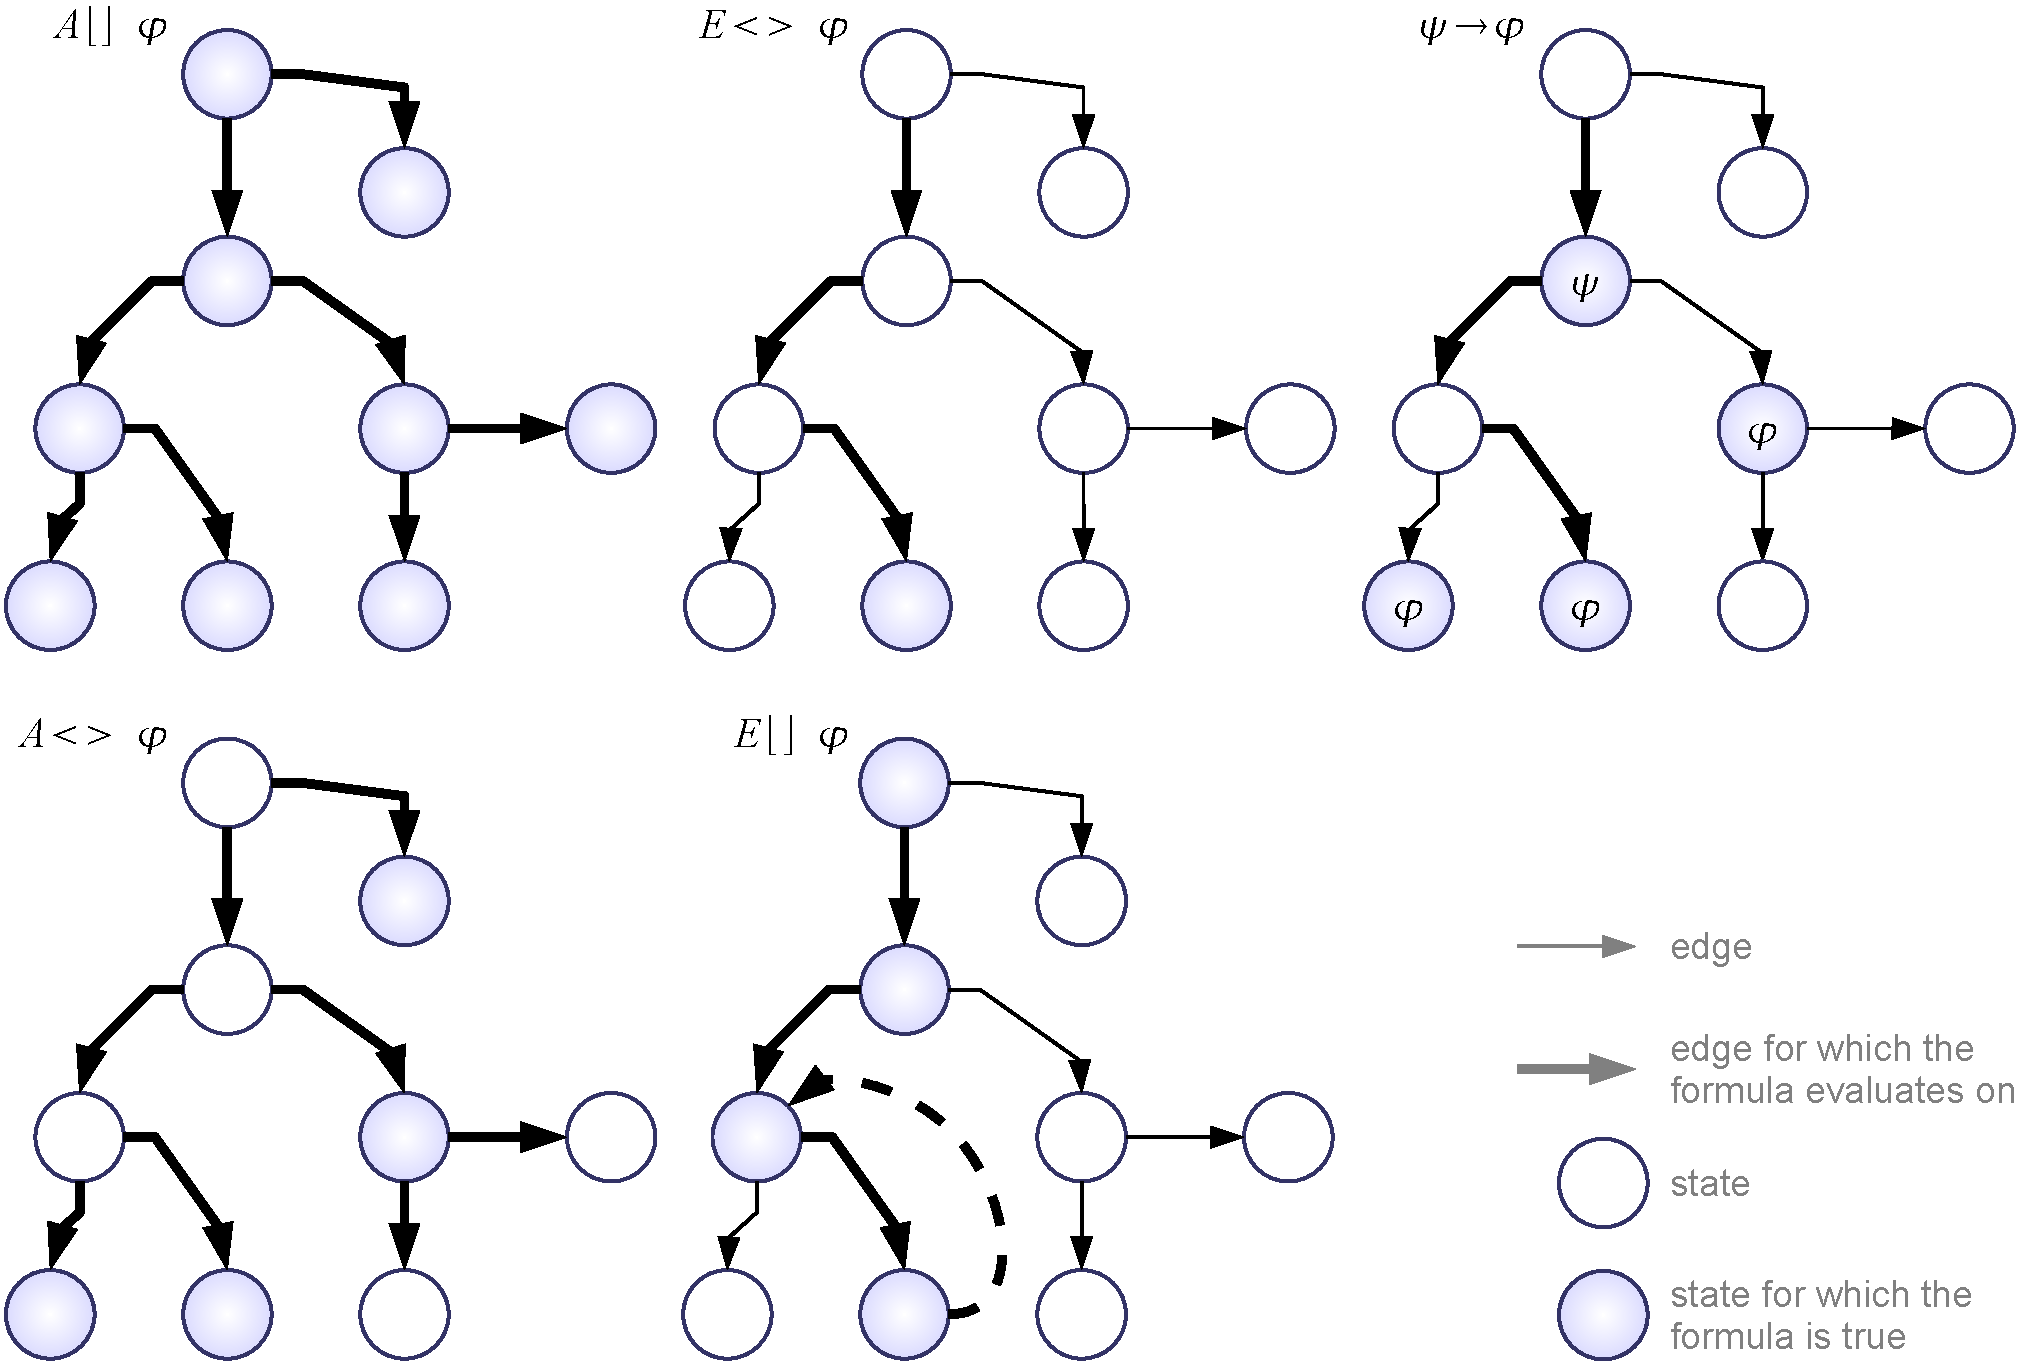
\includegraphics[width=\textwidth]{content/timed-automata/uppaal-path-formulae}
    \begin{flushright}
    	\textit{(source: \cite{UPPAAL})}
    \end{flushright}
    \caption{The path formulae that UPPAAL supports.}
    \label{fig:uppaal-path-formulae}
\end{figure}

We summarize here the types of formula that can be defined for queries in UPPAAL as detailed in \cite{UPPAAL}. We will use Figure~\ref{fig:uppaal-path-formulae} to illustrate them. To begin with, we need \emph{state formula}. Such a formula can be made from clock constraints (e.g., $(x < 3.75) \wedge (y \geq 5)$) and tests that check if a system is in a given location or not (e.g., $P.l$ is true when the system $P$ is currently in the $l$ location). By combining them using boolean conjunctions and disjunctions, it is possible to define complex state formulae such as $\varphi = (x < 3.75) \wedge (y \geq 5) \wedge P.l$. There is also a special state formula $\mathtt{deadlock}$ that is true when neither the current extended state $(l, v)$ offers an outgoing action transition nor there exists a time successor $(l, v')$ that does so. Using state formulae as a basis, the path formulae that can be expressed have been summarized in Table~\ref{tab:uppaal-path-formulae}.\\

\begin{table}[htbp]
\footnotesize
\centering
\begin{tabular}{|p{3cm}|p{7cm}|p{2cm}|}
  
  \hline
  
  \textit{Formula} &
  \textit{Semantic} &
  \textit{Analysis} \\
  
  \hline
  
  $E\Diamond \varphi$ &
  There exists a path to a state $(l, v)$ that verifies $\varphi$. &
  Reachability \\
  
  \hline
  
  $A\Box \varphi$ &
  Every reachable state $(l, v)$ satisfies $\varphi$. &
  Safety \\
  
  \hline
  
  $E\Box \varphi$ &
  There exists a path to a state $(l, v)$ with no outgoing transition that satisfies $\varphi$, or there exists an infinite path where $\varphi$ is satisfied by all states at some point. &
  Safety \\
  
  \hline
  
  $A\Diamond \varphi$ &
  For every possible path, there exists a state $(l, v)$ such that $\varphi$ is satisfied. &
  Liveness \\
  
  \hline
  
  $\varphi \rightarrow \psi$, or equivalently $A\Box (\varphi \Rightarrow A\Diamond \psi)$ &
  Given a state $(l_1, v_1)$ satisfying $\varphi$, every path starting from it contains a state $(l_2, v_2)$ such that $\psi$ is satisfied. &
  Liveness \\
  
  \hline
  
\end{tabular}
\caption{Semantics of the path formulae supported by UPPAAL (a subset of TCTL).}
\label{tab:uppaal-path-formulae}
\end{table}

Going back to the examples of verifications that we expressed as \emph{property 1} and \emph{property 2} on Figure~\ref{fig:light-verification-inclusion}, the properties can be checked by UPPAAL using the following formulae:
\begin{itemize}
  
  \item \emph{property 1}: $E\Diamond (\mathsf{Model.off \wedge x = 10})$ (the location $\mathsf{Model.off}$ is reachable while the clock $x$ has a valuation of 10)
  
  \item \emph{property 2}: $E\Diamond (\mathsf{Model.off \wedge x = 1})$ (there is a path to a state in the LTS of $\mathsf{Model}$ such that the current location is $\mathsf{Model.off}$ and the current valuation of the clock $x$ is 1).
  
\end{itemize}
UPPAAL evaluates the first property to \texttt{true} and the second one to \texttt{false}. Please note that ``undesirable'' properties (i.e., the ones that should normally evaluate to \texttt{false}) are expressed \emph{positively} in UPPAAL (as opposed to \emph{negatively} using a boolean negation operator).\\

UPPAAL supports a subset of TCTL. which provides more path formulae. Also, TCTL allows nested path formulae, something that UPPAAL does not support.\\

% ........................................................................... %

\subsection{UPPAAL tools}

% ........................................................................... %

\begin{figure}[htbp]
    \centering
    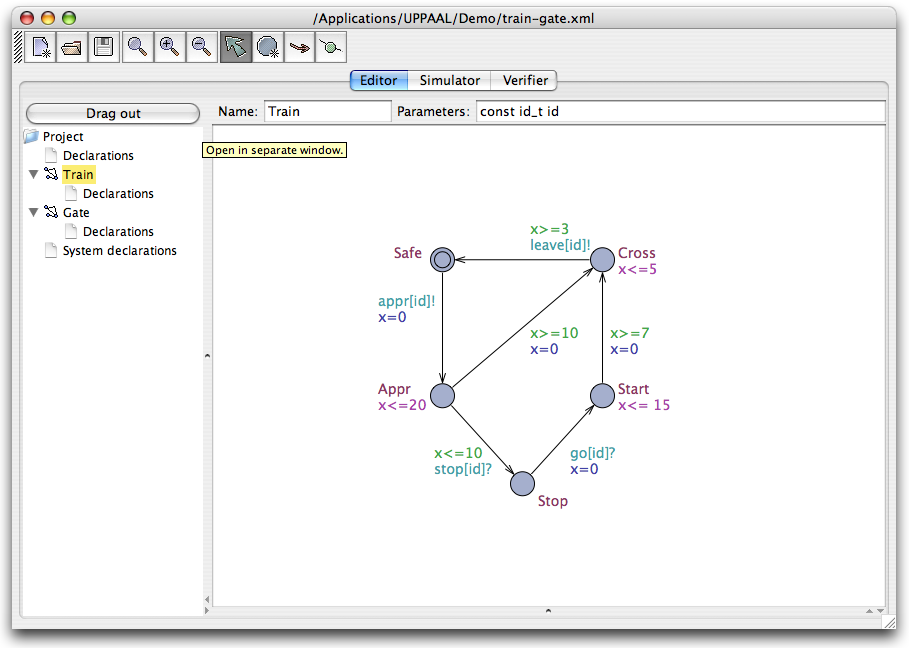
\includegraphics[width=\textwidth]{content/timed-automata/uppaal-1}
    \caption{UPPAAL: modeling environment.}
    \label{fig:uppaal-1}
\end{figure}

UPPAAL comprises two main components:
\begin{enumerate}
  
  \item a command-line model checker called \emph{verifyta}, written in C and ported to Unix variants (Linux, *BSD), Windows and Mac OS X, and
  
  \item a graphical user interface (GUI) written in Java.
  
\end{enumerate}
The UPPAAL GUI (see Figure~\ref{fig:uppaal-1}) is a comprehensive environment for modeling, simulating and verifying systems represented as timed automata. The editor allows to define a set of (usually interacting) systems (e.g., the gate, barrier controller and train systems of the examples found in \cite{RADLD94} or the light controller of Figure~\ref{fig:light-verification-inclusion}).\\

\begin{figure}[htbp]
    \centering
    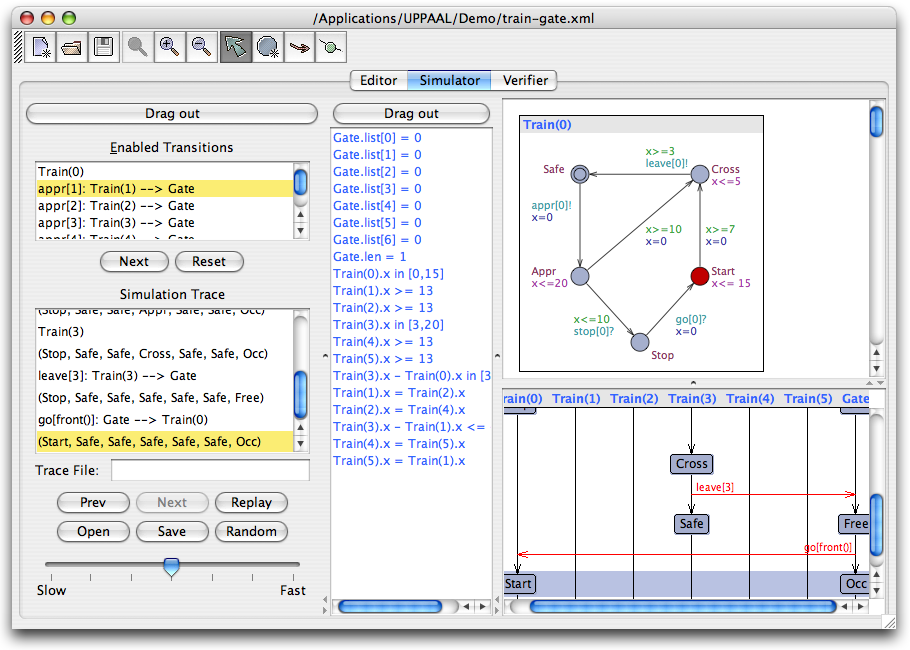
\includegraphics[width=\textwidth]{content/timed-automata/uppaal-2}
    \caption{UPPAAL: simulation environment.}
    \label{fig:uppaal-2}
\end{figure}

The simulator component (see Figure~\ref{fig:uppaal-2}) allows users to simulate the execution of the systems to see which switches are taken, what are the clocks valuation ranges at each step and so on. The simulation can be run automatically by the tool: when several switches can be enabled from a given location, the next switch is selected randomly. Otherwise, the user can select which switch should be taken next at each step. In the later case, the simulator acts as a kind of step-by-step debugger as found for traditional programming using languages such as C/C++, Java and so on.\\

\begin{figure}[htbp]
    \centering
    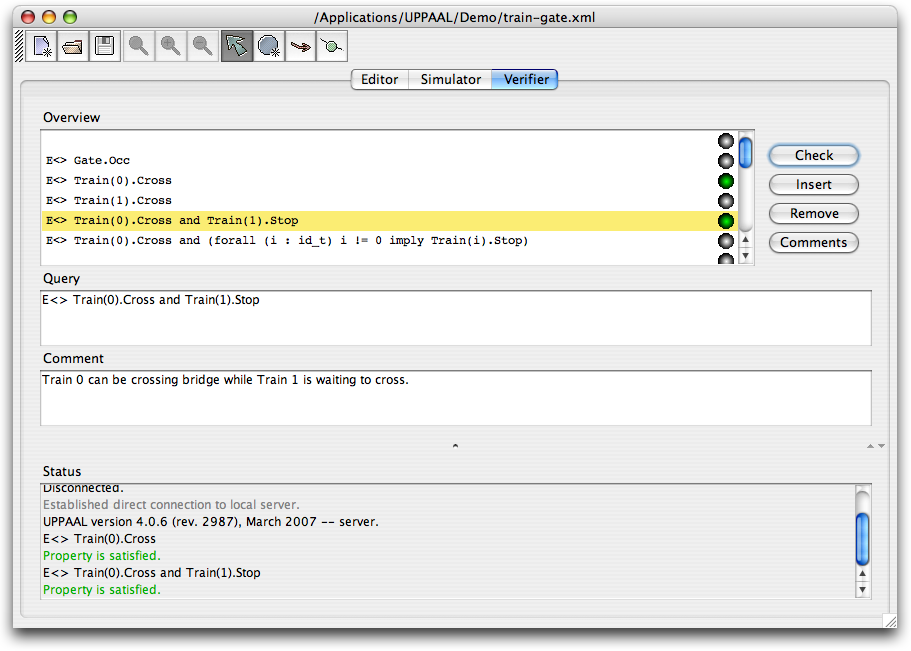
\includegraphics[width=\textwidth]{content/timed-automata/uppaal-3}
    \caption{UPPAAL: verification environment.}
    \label{fig:uppaal-3}
\end{figure}

Finally, the verification component (see Figure~\ref{fig:uppaal-3}) allows to perform verifications by encoding requests in (timed) temporal logics. In fact, this component is directly using the command-line \emph{verifyta} tool to perform the verifications.\\

% ........................................................................... %

